\documentclass[12pt, a4paper]{article}

% --- ПРЕАМБУЛА ---
\usepackage[utf8]{inputenc}
\usepackage[russian]{babel}
\usepackage{amsmath} % Расширенные математические возможности
\usepackage{amssymb} % Дополнительные математические символы
\usepackage{graphicx} % Для вставки изображений
\usepackage{geometry} % Для настройки полей
\geometry{a4paper, total={170mm,257mm}, left=20mm, top=20mm}

% Определение команд для Математического ожидания, Дисперсии и Ковариации
\DeclareMathOperator{\E}{E}
\DeclareMathOperator{\D}{D}
\DeclareMathOperator{\cov}{cov}

\begin{document}

% --- НАЧАЛО ТЕКСТА ЛЕКЦИИ ---

\section*{Вступление}

Каждый, кто хоть раз работал с осциллографом или вольтметром, замечал, что напряжение или сила тока в цепи никогда не принимают строго определенное значение, они постоянно меняются, <<пляшут>> вокруг некоторого значения. Это так называемые \textbf{шумы} или флуктуации, которые присутствуют в цепях, как и в любых других физических системах. Для описания шумов нам понадобится математический аппарат теории вероятностей, так как шум представляет собой случайный процесс, поэтому будет разумно для начала вспомнить необходимую математическую теорию.

\section*{Необходимые знания из теории вероятностей}

\subsection*{Характеристики случайной величины}

\textbf{Случайная величина} — это переменная, которая в результате случайного эксперимента принимает одно из множества возможных числовых значений. Мы не можем предсказать точное значение, которое она примет, но можем описать вероятность появления тех или иных значений. Далее мы будем говорить о непрерывных случайных величинах. Случайная величина полностью описывается своей плотностью вероятности $f(x)$.

\textbf{Математическое ожидание} — характеристика случайной величины, которая определяется формулой:
\[
\E[X] = \int\limits_{-\infty}^{\infty}x \cdot f(x)dx
\]
Математическое ожидание имеет смысл среднего взвешенного.

\textbf{Дисперсия} определяется через матожидание:
\[
\D[X] = \E[(X - \E[X])^2]
\]
Дисперсия является мерой разброса случайной величины. Можно переписать в другом виде:
\[
\D[X] = \E[X^2] - (\E[X])^2
\]
Иногда это бывает полезно. Дисперсия имеет размерность квадрата величины, поэтому иногда бывает удобнее пользоваться \textbf{среднеквадратичным отклонением}:
\[
\sigma_X = \sqrt{\D[X]}
\]
Случайные величины $X$ и $Y$ называются \textbf{независимыми}, если для их математических ожиданий выполняется следующее тождество:
\[
\E[XY] = \E[X]\E[Y]
\]
Однако более интуитивное определение получится, если переписать это выражение:
\[
\E[X] = \E[X|Y] = \frac{\E[XY]}{\E[Y]}, \qquad \E[Y]= \E[Y|X] = \frac{\E[XY]}{\E[X]}
\]
Получаем определение условной вероятности. Отсюда видно, что случайные величины независимы, если информация о значении одной из них не дает дополнительной информации о величине другой.

\textbf{Совместное распределение двух случайных величин.} Предположим, что у нас есть случайная величина $\zeta$, которая является функцией от двух других случайных величин $\xi$, $\eta$.
\[
\zeta = \phi(\xi, \eta)
\]
Каждая случайная величина обладает своим распределением, поэтому для того, чтобы посчитать, например, матожидание $\zeta$, нужно рассматривать совместное распределение $\rho(x, y)$:
\[
\E[\zeta] = \iint \phi(x, y)\rho(x, y)dxdy
\]

\textbf{Ковариация} случайной величины определяется следующей формулой:
\[
\cov(X, Y) = \E[(X - \E[X])(Y - \E[Y])] = \E[XY] - \E[X]\E[Y]
\]
Ковариация показывает, насколько синхронно изменяются две величины. Если ковариация равна нулю, величины называют некоррелированными (не путать с независимостью!). \textbf{Коэффициент корреляции} представляет из себя нормированную ковариацию:
\[
\rho_{XY} = \frac{\cov(X,Y)}{\sigma_X\sigma_Y} \in [-1, 1]
\]

\subsection*{Характеристики случайного процесса}

Теперь поговорим об основном объекте нашего исследования. \textbf{Случайный процесс} $X(t, \omega)$ — это функция двух переменных:
\begin{enumerate}
    \item $t$ (Обычно время) — аргумент из некоторого множества $T$.
    \item Элементарного исхода $\omega$, принадлежащего пространству элементарных исходов $\Omega$.
\end{enumerate}

Представьте себе завод по производству генераторов шума. Возьмем все произведенные на заводе генераторы и одновременно включим их. Аргумент $\omega$ отвечает за выбор генератора шума, а $t$ — за выбор момента времени, в который мы смотрим на значения генератора. То есть конкретный генератор символизирует реализацию случайного процесса, которая является функцией времени. Если мы фиксируем время и смотрим значения на разных генераторах, то получаем случайную величину.

% --- МЕСТО ДЛЯ КАРТИНКИ ---
% Поместите файл generators.png в ту же папку, что и ваш .tex файл
\begin{figure}[h!]
    \centering
    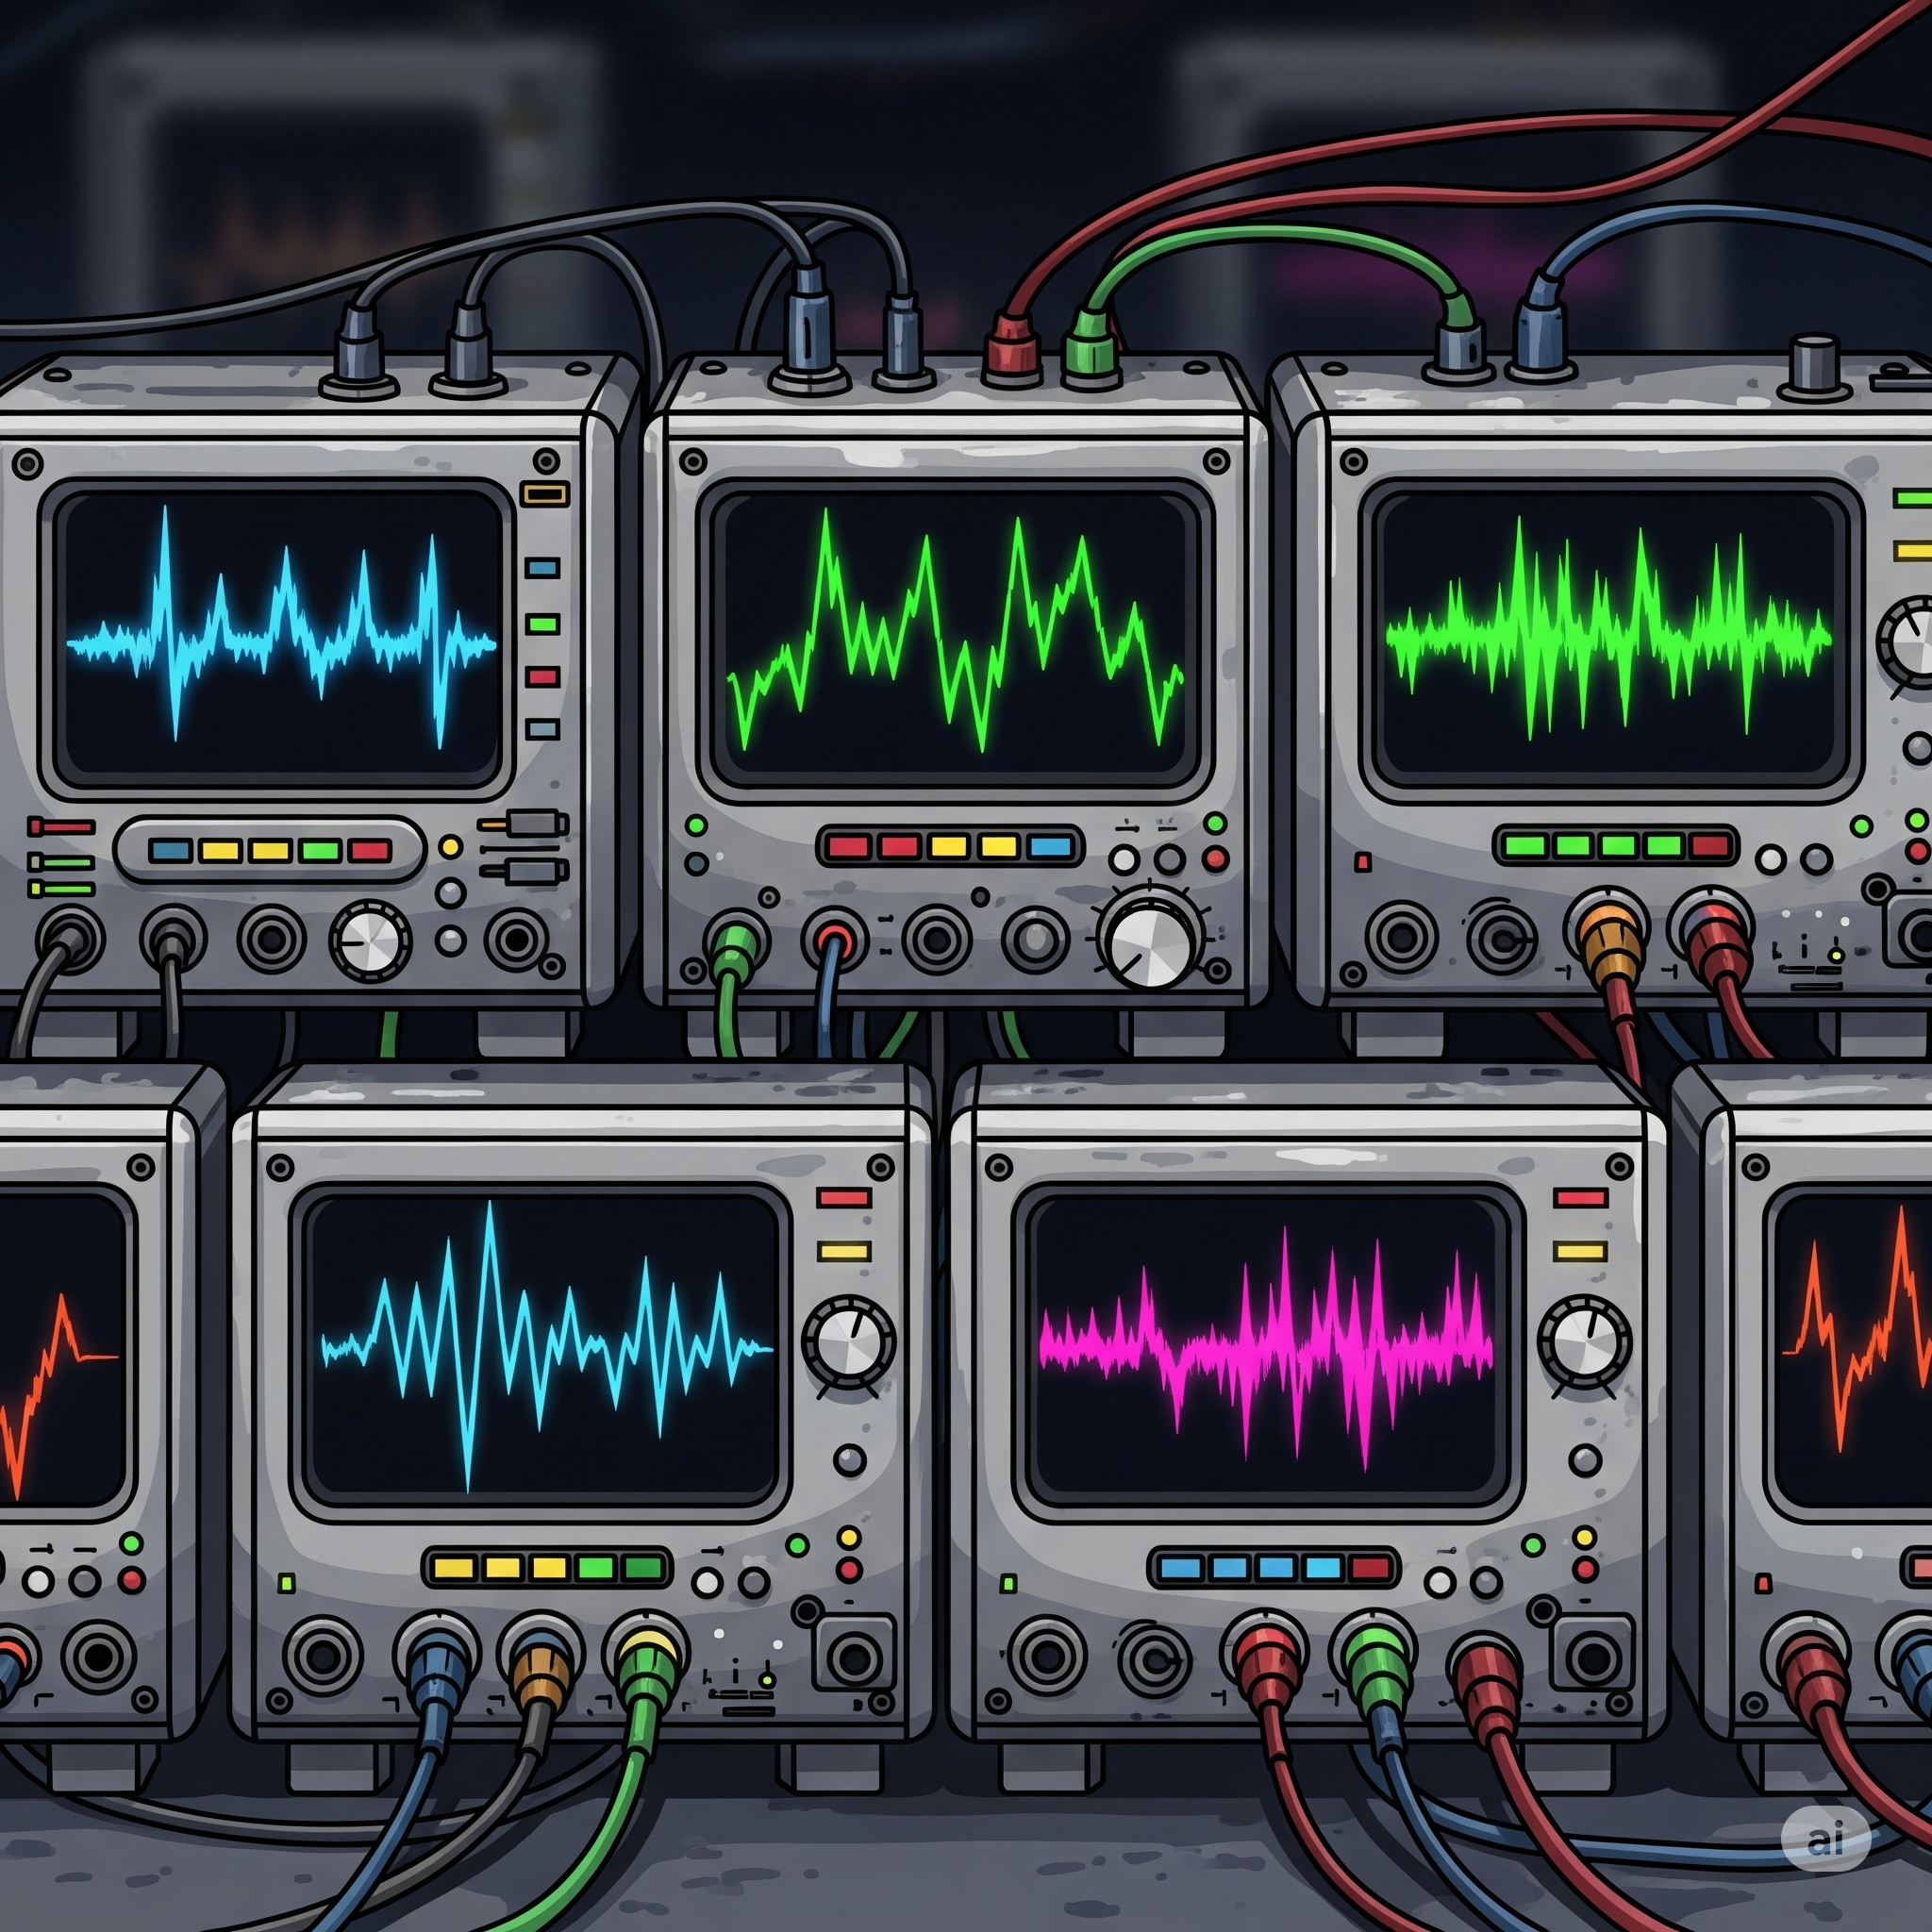
\includegraphics[width=0.6\textwidth]{generators.png}
    % \caption*{Иллюстрация: ансамбль реализаций случайного процесса.} % Раскомментируйте, если нужна подпись
\end{figure}

Здесь стоит сделать важное замечание. Далее мы будем рассматривать только \textbf{эргодические} случайные процессы. Все реальные шумы относятся к этому классу. Процесс называется эргодическим, если усреднение по времени одной-единственной реализации дает тот же результат, что и усреднение по всему ансамблю в один момент времени. То есть если мы возьмем один-единственный генератор шума с нашего завода и вычислим среднее, то получим тот же результат, как если бы усредняли по значениям всех генераторов в фиксированный момент времени.

Эргодический процесс всегда является также и стационарным. Это значит, что его вероятностные характеристики не зависят от времени. Разница между стационарностью и эргодичностью хоть и не велика, но присутствует. Не каждый стационарный процесс является эргодическим.

Если мы хотим вычислить матожидание или дисперсию для стационарного процесса, мы можем просто зафиксировать произвольный момент и вычислить их через формулу для случайной величины. Плотность вероятности в силу стационарности не зависит от времени.
\[
\E[x] = \int x \rho(x)dx
\]
Если же процесс является эргодическим, то вычисление вероятностных характеристик сводится к <<усреднению по времени>>:
\[
\E[x] = \lim\limits_{T\rightarrow\infty} \frac{1}{2T}\int\limits_{-T}^{T}x(t)dt, \qquad \D[x] = \lim\limits_{T\rightarrow\infty} \frac{1}{2T}\int\limits_{-T}^{T}[x(t)-\E[x]]^2dt
\]
Для случайных процессов также вводится корреляция. Если присутствует два случайных процесса, то рассматривается \textbf{взаимная корреляционная функция}:
\[
\langle x, y \rangle (\tau) = \E\left[ x(u)y(\tau-u) \right]
\]
Для одного сигнала рассматривается \textbf{автокорреляция}:
\[
\langle x, x \rangle (\tau) = \E\left[ x(u)x(\tau-u) \right]
\]
Пользуясь эргодичностью, можно аналогично матожиданию и дисперсии заменить усреднение по выборкам на усреднение по времени отдельной реализации:
\[
\langle x, y \rangle (\tau) = \lim\limits_{T \rightarrow\infty}\frac{1}{T}\int\limits_{-T/2}^{T/2}x(u)y(u-\tau)du
\]
(И аналогично для автокорреляции). Заметим схожесть формулы автокорреляции с формулой свертки (отличие лишь в знаке при $\tau$, поэтому для корреляции коммутативность, в отличие от свертки, не выполняется).

Теперь мы готовы к изучению теории шумов.

\section*{Шум}

Как уже было сказано выше, шум является эргодическим, а значит стационарным случайным процессом. Тогда можно вычислять вероятностные характеристики аналогично вычислению характеристик случайных величин. Мощностью шума называется следующее выражение:
\[
\sigma^2 = \E[n^2] = \int n^2 p(n)dn,
\]
где $p(n)$ — плотность распределения. Такое обозначение мощности шума введено для того, чтобы сам символ $\sigma$ обозначал \textbf{эффективное значение шума}. Пользуясь эргодичностью, сведем вычисление мощности к интегрированию по времени:
\[
\sigma_T^2 = \frac{1}{T}\int\limits^{T/2}_{-T/2}n^2(u)du \approx \frac{1}{N}\sum\limits_{i=1}^N n^2(u_i)
\]
Таким образом можно вычислить приблизительное значение мощности экспериментально. Автокорреляцию шума называют просто \textbf{корреляцией шума} и обозначают таким символом:
\[
\overline{n^2(t)} = \langle n, n \rangle (t) = \E[n(u)n(t-u)]
\]
Заметим, что при $t=0$ корреляция шума равна его мощности.

Для нескольких шумов вводится понятие взаимной корреляции, которое полностью совпадает с взаимной корреляцией случайных процессов:
\[
\langle n_1, n_2 \rangle (t) = \lim\limits_{T \rightarrow\infty}\frac{1}{T}\int\limits_{-T/2}^{T/2}n_1(u)n_2(u-t)du
\]
Далее мы будем считать, что все шумы, порожденные разными физическими механизмами, некоррелированны.

\section*{Спектральная плотность шума}

Это каноническая форма преобразования Фурье. Пусть будет тут.
\[
\mathcal{F}\left[f\right](\omega) = \text{v.p.}\frac{1}{\sqrt{2\pi}}\int\limits_{-\infty}^{\infty}f(t)e^{-i\omega t} dt
\]
Спектральная плотность шума $S_n(f)$ (или $n^2(f)$) определяется следующим образом.
\[
\frac{S_n(f)}{2} =\int\limits_{-\infty}^{\infty}\overline{n^2(t)}e^{-j2\pi ft} dt
\]
Обсудим, откуда берется двойка. Если мы посмотрим на определение корреляции шума $\overline{n^2(t)}$, то увидим, что это четная действительная функция. Как известно, в таком случае ее фурье-образ также будет вещественной четной функцией.
\[
\int\limits_{-\infty}^{\infty}\overline{n^2(t)}e^{-j2\pi ft} dt = \int\limits_{-\infty}^{\infty}\overline{n^2(t)}(\cos(2\pi ft) - j\sin(2\pi ft))dt
\]
Если спектр является четной функцией, значит, ее отрицательная ось частот не несет в себе дополнительной информации. Таким образом, ее можно отбросить. Однако для сохранения полной мощности стоит удвоить положительную часть. В этом и кроется смысл двойки: $S_n(f)$ — это \textbf{односторонняя} спектральная плотность.

Преобразование Фурье обратимо, значит, можно выразить корреляцию через спектральную плотность:
\[
\overline{n^2(t)} = \dots
\]

\subsection*{Путаница определений}
Итак, мы уже понимаем, что спектральная односторонняя плотность шума — это удвоенное преобразование Фурье от корреляции. Какую размерность имеет $\overline{n^2(t)}$?

% --- КОНЕЦ ТЕКСТА ЛЕКЦИИ ---

\end{document}